% !TeX spellcheck = de_DE
\documentclass[a4paper,11pt,singlespacing]{article}

\usepackage{setspace}
\usepackage[utf8]{inputenc}
\usepackage[T1]{fontenc}
\usepackage{graphicx}
\usepackage{color}
\usepackage{hyperref}
\usepackage{listings,xcolor}
\usepackage{pdfpages}
\usepackage{float}

\renewcommand{\contentsname}{Inhaltsverzeichnis}
\renewcommand{\figurename}{Abbildung}

\graphicspath{ {./images/} }


\begin{document}
    
 \setlength{\parindent}{0ex}
    	
\begin{titlepage}
    \begin{center}
    
\includegraphics[scale=0.3]{rwu_logo_hor-lila-cyan_rgb_0}
        \vspace*{1.5cm}
        
        \Huge
        \textbf{WLAN-AP mit regelmäßigem PSK-Tausch und QR-Code Anmeldung}
            
        \vspace{1.4cm}
        \normalsize
        Luca Asmus, 29994\\ Marius Würstle, 29853\\Rolf Wiersch, 29837
            
        \vspace{1.0cm}
        
        %\vfill
          \normalsize
        \textbf{Zusammenfassung}\\
    	Das Ziel dieses Projekts war es, die Sicherheit im eigenen Gast-WLAN zu gewährleisten, unter Berücksichtigung der Faulheit und Bequemlichkeit vieler Endnutzer. Der pre-shared Key eines WLANs wird in den meisten Netzwerken einmal oder nie geändert. Dadurch können Gäste dauerhaften Zugang zum Netzwerk behalten, obwohl das nicht erwünscht ist. Ein weiteres Problem ist die Umständlichkeit einen sicheren pre-shared Key zu verwenden. Es führt zu unangenehmen Mehraufwand eine kryptische und lange Zeichenkette auf Endgeräten einzugeben. Gelöst wurde dies durch einen eigenen Access Point für Gäste. Über diesen wird der Zugriff ins Internet geleitet. Der pre-shared Key wird einmal die Woche oder manuell neu erzeugt und auf einem Display ausgegeben. Die Ausgabe erfolgt in Form eines QR - Codes und in Klartext.   \\
        
        \vspace{2.0cm}
        December 12, 2020
        
        \vspace{0.8cm}
          
            
    \end{center}
\end{titlepage}
    	

    	\pagestyle{empty}
    	\tableofcontents
    	\cleardoublepage
    	\pagestyle{plain}

    \section{Motivation}
    	Der Hauptgrund für dieses Projekt war es die Sicherheit im eigenen Gast-WLAN zu gewährleisten, unter Berücksichtigung der Faulheit und Bequemlichkeit vieler Endnutzer. \\ \\
    	Wenn Gäste in der heimischen Wohnung auftauchen, ist der Wunsch nach freiem WLAN meist sehr groß. Bedeutet, der pre-shared key muss abgelesen und den Gästen bekannt gemacht werden. Folgend muss dieser umständlich von Hand eingegeben werden. Um hierbei Sicherheit zu gewährleisten, ist dieser meist länger und kryptisch gewählt. Dies führt oft zur falschen Eingabe bzw. Mehrversuchen und darauf folgenden Ärger darüber. Weiterhin ist es vom Gastgeber nicht immer erwünscht, dass die Gäste nach der Verabschiedung den Zugriff zum WLAN behalten. \\ \\
    	Da die geschilderten Umstände den Verfassern dieses Dokumentes nicht fremd sind, soll mit diesem Projekt eine eigenständige Lösung erstellt werden. Der Fokus liegt auf einfacher Bedienung und komfortabler Sicherheit. Weiterhin wird für die Sicherheit auf fertige Endprodukte von Drittanbietern verzichtet. 
    			
    \section{Grundlagen Hard- und Software}
      	In den folgenden Abschnitten werden Hardware und Software genauer erläutert. Im Glossar am Ende der Projektarbeit können weitere Erklärungen bzw. Akronyme entnommen werden.
      	\subsection{Hardware}
    		\subsubsection{Raspberry Pi}
    			Der Raspberry Pi wurde für junge Menschen entwickelt, um ihnen eine preisgünstige Möglichkeit zu bieten, sich mit der Informatik zu beschäftigen. Der Einplatinencomputer ist etwa kreditkartengroß und kam Anfang 2012 auf den Markt. Er ermöglicht einen schnellen und praktischen Weg um Wissen in den Bereichen Programmieren und Hardware zu erlangen. Zudem ist er vielseitig einsetzbar.
    			\begin{figure}[H]
    				\centering
	    			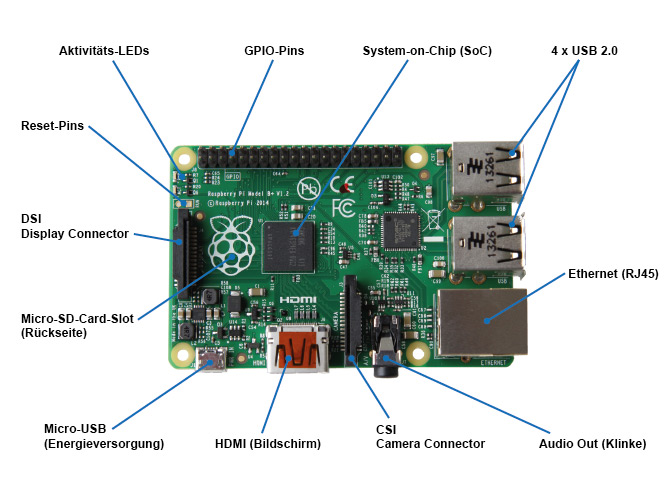
\includegraphics[scale=0.5]{raspberry_pi_3b}
	    				\caption{Raspberry Pi 3b - Quelle: \cite{Picture_Raspberrypi3b} }
	    				\label{raspberrypi3b}
				\end{figure}
				Technische Spezifikationen des Raspberry Pi 3b:
				\begin{itemize}
					\item Quad Core 1.2GHz Broadcom BCM2837 64bit CPU
					\item 1GB RAM
					\item BCM43438 wireless LAN and Bluetooth Low Energy (BLE) on board
					\item 100 Base Ethernet
					\item 40-pin extended GPIO
					\item 4 USB 2 ports
					\item 4 Pole stereo output and composite video port
					\item Full size HDMI
					\item CSI camera port for connecting a Raspberry Pi camera
					\item DSI display port for connecting a Raspberry Pi touchscreen display
					\item Micro SD port for loading your operating system and storing data
					\item Upgraded switched Micro USB power source up to 2.5A  \cite{Quote_Raspberrypi3b}
				\end{itemize}
			\subsubsection{Raspberry Pi Shield - Display LCD-Touch, 3,2in}
				Der Touchscreen wertet den Raspberry Pi zu einem vollwertigen Touch-PC auf. Für zusätzliche Funktionen besitzt der Display 3 Buttons an der Seite, welche einfach über die GPIO Pins eingelesen werden können.
				\begin{figure}[H]
					\centering
					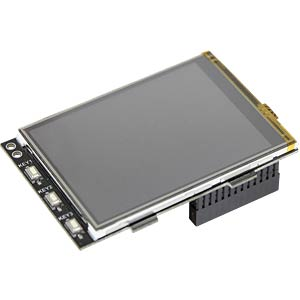
\includegraphics[scale=0.5]{touch_display}
					\caption{Touchscreen Display für den Raspberry Pi - Quelle: \cite{Picture_touchdisplay}}
					\label{touchdisplay}
				\end{figure}
				Technische Spezifikationen unseres Raspberry Pi Shield - Display LCD-Touch, 3.2in:
				\begin{itemize}
					\item Display 8,13cm (3,2")
					\item Auflösung 320 x 240 Pixel
					\item LED-Hintergrundbeleuchtung
					\item 3 frei belegbare Taster (angebunden an GPIO12, 16, 18)
					\item SPI-Schnittstelle
					\item Touchscreen Technologie resistiv
				\end{itemize}
    			
    	\subsection{Software}
    		\subsubsection{balenaEtcher}
    			Programm mit dem ein OS auf eine SD Karte geflasht werden kann.
    		\subsubsection{hostapd}
        		Mit  ist es möglich Geräte, die ein WLAN-Modul besitzen, als Access Point zu betreiben. Jedoch können keine Einstellungen im Bereich IP und Routing vorgenommen werden. Die Software ist nur für das Erstellen eines "wireless Ethernet switches" zuständig. \cite{Quote_hostapd1} 
    		\subsubsection{dnsmasq}
        		Geräte in einem Netzwerk benötigen zur Kommunikation eine IP Adresse und einen DNS Server für die Namensauflösung. Deshalb muss in diesem Projekt ein DHCP und DNS erstellt werden. Von diesen bekommen die Endgeräte ihre IP Konfiguration im WLAN. Die Software dnsmasq wird in diesem Projekt verwendet, um dies zu ermöglichen.
    		\subsubsection{netfilter-persistent und iptables-persistent}
        		Für die Durchführung des Projektes ist es nötig iptables-Regeln anzulegen. Diese sollten nach einem Neustart nicht neu angelegt werden müssen. Deshalb wurden die Pakete netfilter-persistent und iptables-persistent installiert. Damit können die Regeln in eine Datei abgespeichert und beim Neustart automatisch geladen werden.
        	\subsubsection{Bash}
        		Im Projekt wird Bash benutzt um die einzelnen Python Skripte aufzurufen, Infos aus Konfigurationsdateien auszulesen und schnelle Änderungen an Diesen vorzunehmen. Bash ist als Standardshell bei Raspberry Pi OS Lite vorinstalliert. 
    		\subsubsection{Cron}
				Cron ermöglicht das zeitbasierte Ausführen des Bash Skripts. So kann beispielsweise jeden Montag um 03:00 Uhr nachts das Passwort automatisch geändert werden.
			\subsubsection{fim}
				fim ermöglicht es Bilder oder andere Media Dateien im Terminal anzuzeigen. In diesem Fall wird der QR-Code als .png erzeugt und mithilfe von fim angezeigt. \cite{Quote_man_fim}
    		\subsubsection{Python 3.7}
    			Für die Skripte zur Passwortgenerierung, QR-Code Generierung und zum Einlesen der Buttons wird die Sprache Python verwendet. Python 3.7 ist bei Raspberry Pi OS Lite  vorinstalliert und erleichtert durch verschiedene Bibliotheken die Umsetzung des Projektes.
    			\subsubsection{pyqrcode}
    				Das Modul pyqrcode wird dafür benutzt, möglichst einfach und frei QR-Codes zu erzeugen. Zum Erzeugen des Codes benötigt sie nur die Parameter die enthalten sein sollen. \cite{Quote_pyqrcode}
    			\subsubsection{GPIO zero}
    				Das Modul GPIO zero wird in diesem Projekt für das Einlesen der einzelnen Buttons genutzt, die bereits in dem Display integriert sind. Das Mapping der Buttons wird auch in der Anleitung des Displays erklärt. (Button1 = PIN12/GPIO18) \cite{Quote_gpio_zero}
    	
    	
    \section{Problemstellung}
    	Vielen Endnutzern ist die eigene Bequemlichkeit sehr wichtig. Daraus resultiert, dass der pre-shared Key eines WLANs in den meisten Netzwerken einmal oder nie geändert wird. Dadurchk önnen Gäste dauerhaften Zugang zum Netzwerk behalten, obwohl das nicht erwünscht ist. Dies hat zur Folge, dass sich sobald einmal das Passwort bewusst/unbewusst weitergegeben wurde, jeder mit dem Access Point verbinden kann. Negative Auswirkungen könnten sich äußern in Form von Missbrauch des Internetzuganges oder durch Angriffe auf das interne Netzwerk.Ein weiteres Problem ist die Umständlichkeit einen sicheren pre-shared Key zu verwenden. Es führt zu unangenehmen Mehraufwand eine kryptische und lange Zeichenkette auf Endgeräten einzugeben bzw. zu merken, den viele Endnutzer nicht eingehen wollen. Deshalb werden oft einfache pre-sharedKeys in Form von z.B Wortkombinationen verwendet. Dies hat zur Folge,dass der Zugang einfacher geknackt werden kann.
    	
   \section{Anforderungsanalyse}
    		Im Folgenden werden die verschiedenen Anforderungen genauer beschrieben.
			\subsection{Funktionale Anforderungen}
			Funktionale Anforderungen sind Anforderungen, die notwendig für die Umsetzung des Projektes sind.
            \subsubsection{Funktionaler Accesss Point}
                Um einen Zugriffspunkt für die Endnutzer ins Netzwerk zu schaffen, muss passende Hardware gefunden und konfiguriert werden. Hierauf wird ein Access Point mit gängiger Funktionalität erstellt.\\ 
                Die Hardware sollte für ihre Aufgaben passend dimensioniert sein. Ebenso sollte sie ein geeignetes WLAN-Modul besitzen um ein eigenes WLAN aufspannen zu können. Am Besten ist es, wenn dieses die heutzutage gängigen Funkstandards unterstützt.\\\\
                Weiterhin müssen sich die Endnutzer im WLAN anmelden und kommunizieren können. Unter anderem wird ein DNS und DHCP Server benötigt. Ohne diesen kann keine Kommunikation im Funknetzwerk entstehen. Grund ist die fehlende IP-Konfiguration der Endgeräte.
                \subsubsection{Zugriff ins Netzwerk}
                    Ohne Internet Zugriff ist zwar eine Anmeldung beim Access Point möglich, aber nicht sinnvoll.
                    Deshalb muss gewährleistet werden, dass der Datenverkehr vom Access Point weitergeleitet wird und nicht geblockt wird. Natürlich soll dieser auch wieder zurückgeleitet werden. Am Besten besitzt die Hardware außerdem einen LAN Anschluss. Dieser kann als Verbindung zur schon bestehenden Infrastruktur dienen.
                \subsubsection{Sicherer Key}
                    Beim erstellen des Key muss beachtet werden, dass dieser auch sicher ist. Es soll unwahrscheinlich sein diesen in seinem gültigen Zeitraum knacken zu können. Deshalb muss ein Konzept zur Erstellung eines sicheren Key erstellt und umgesetzt werden. 
    			\subsubsection{Automatisches Wechseln des Key}
    			    Es soll möglich sein das sich der Key vollautomatisch in einem gewissen Zeitraum ändert. Folglich muss ein Skript erstellt werden, welches den Key austauschen kann.
    			\subsubsection{Ausgabe des Key}
		            Die Endnutzer müssen über den neu erstellten Key benachrichtigt werden. Zu beachtet ist, dass die Darstellung so komfortabel wie möglich umgesetzt wird. Es soll kein zu großer Mehraufwand entstehen. Weitere Hardware in Form eines Bildschirm zu Darstellung muss angeschlossen werden.
		           
		            
			\subsection{Optionale Anforderungen}
			    In diesen Abschnitt werden Anforderungen beschrieben, die nicht für die grundlegende Funktionalität benötigt werden.
                \subsubsection{Manueller Wechsels des Key}
                    Wenn es gewünscht es soll es möglich sein den Key manuelle neu erstellen und wechseln zu lassen. Die soll in Form einer physischen Benutzereingabe erfolgen. So wird sichergestellt, dass nur befugte diesen Vorgang anstoßen können. 
                \subsubsection{Energiespar-Konfiguration}
                    Nicht jeder möchte, dass ein Bildschirm ununterbrochen beleuchtet wird. Weiterhin könnte es nicht erwünscht sein, dass das Gast-Wlan 24 Stunden sendet. Deshalb könnte ein Energiesparplan erstellt werden und implementiert werden. Dieser kann die Anschaltzeit des Displays und des Access Points regeln. 
                \subsubsection{Automatisierungs-Skript}
                    In Zukunft könnte es wünschenswert sein, die erstellten Konfigurationen erneut auf anderen Geräten auszuführen. Deshalb könnt ein Automatisierungs-Skript sinnvoll sein. Dies würde Zeitaufwand sparen und könnte ebenso bei veröffentlicht anderen helfen.  

    		\subsection{Priorisierung}
            	Das wichtigste zu Beginn ist, dass die Hardware aufeinander abgestimmt wird. Bedeutet, alle Teile passen zusammen und können angeschlossen werden.
            	Danach muss die Konfiguration des Raspberry Pi zum Access Point erfolgen. Sobald dies funktioniert kann das Generieren des pre-shared Keys und dessen Austausch stattfinden. Folglich wird die Ausgabe des Keys am Bildschirm realisiert. Danach kann dies, um das Generieren des QR-Codes und dessen Ausgabe erweitert werden.\\
            	Wenn diese Punkte voll funktional umgesetzt werden konnten, kann sich um einen automatischen oder manuellen Job (bei Tastendruck) zum Generieren und Austauschen des Keys gekümmert werden.
    	
	\section{Lösungsidee}
    	Ein Lösungsansatz stellt ein sich automatisch oder auf Tastendruck änderbarer pre-shared Key dar. Der Key wird jeden Montagmorgen um 03:00 Uhr automatisch durch einen "Cron-Job" gewechselt. Ein Taster kann zusätzlich betätigt werden, falls das Passwort sofort geändert werden soll. \\
		Der Key wird so gewählt, dass er aus mathematischer Sicht nicht in dem Zeitraum geknackt werden kann, bis automatisch ein neuer erzeugt wird. Durch diese Maßnahme wird die Sicherheit des WLANs verbessert und sicher-gestellt.
		Mit diesem neu generierten Key können sich Endgeräte anmelden und kommunizieren. Hiermit wird das Problem der ungewollten Nutzern gelöst. Diese können sich sobald der Key gewechselt hat, nicht mehr im Netz anmelden. Der Key wird an einem Display in zwei verschiedenen Varianten angezeigt:
		\begin{itemize}
			\item Klartext für Endgeräte ohne Kamera z.B. Laptops
			\item QR-Code zum Scannen für z.B Smartphones
		\end{itemize}
		
		Ürsprünglich war ein RFID/NFC Transponder für die Anmeldung geplant. Es wurde sich für einen QR-Code entschieden, da hier die Möglichkeit des Abgreifens des Keys nicht besteht. In Abbildung  \ref{aufbau} ist der Aufbau des Lösungsansatzes graphisch dargestellt. 

		\begin{figure}[ht]
			\centering
			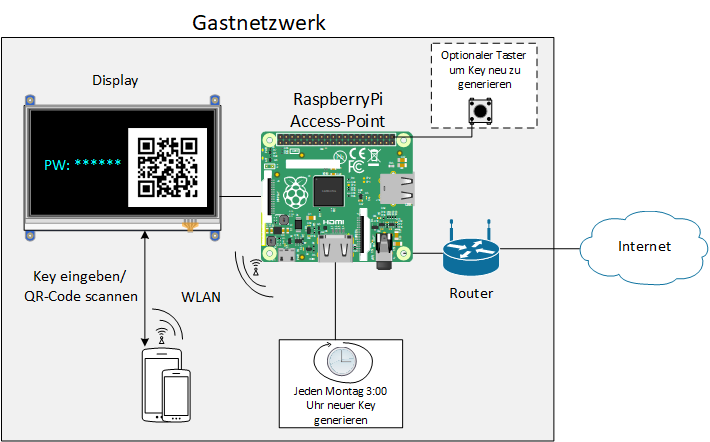
\includegraphics[scale=0.6]{skizze}
				\caption{Aufbau des Gastnetzes}
				\label{aufbau}
		\end{figure}

    	Es ist zu erwähnen, dass sich diese Lösung auf die Umsetzung eines Gastnetzes bezieht. Dieses ist getrennt vom restlichen Heimnetz. Es melden sich dort hauptsächlich mobile Geräte an. Dies führt zu einer hohen Fluktuation an Endgeräten im Netzwerk und ist nicht für stationäre Geräte wie z.B Drucker geeignet.
    
    
    	\subsection{Hardware}
			Für dieses Projekt wird ein Raspberry Pi 3 B benötigt. Grund hierfür ist das integrierte WLAN-Modul, ausreichend Leistung und alle benötigten Anschlüsse sind vorhanden. \\
			Zusätzlich wird eine Mikro-SD Karte zum Laden des Betriebsystems und zur Speicherung der Daten benötigt. \\ \\
			Das Display, welches verwendet wird, muss eine ausreichende Auflösung für die Darstellung des QR-Codes besitzen. Deshalb können keine kleineren und billigeren LCD Anzeigen verwendet werden. Außerdem muss es die Möglichkeit haben entweder externe Taster anzubinden oder schon eigene Taster besitzen.
		
		\subsection{Software}
			Um den Raspberry Pi als Access Point verwenden zu können, müssen zusätzliche Pakete installiert (hostapd) und eine Netzwerkkonfiguration vorgenommen werden. Darunter fällt das Einstellen von DHCP und DNS für die Clients durch "dnsmasq" und Anpassen der IP-Konfiguration. Das Routing erfolgt durch eine neue iptables Regel.\\ \\
		
			Als Skriptsprache empfiehlt sich Python, da es dort sehr viele Libraries gibt, die einiges an Arbeit abnehmen. Zudem kann mit Python auf einfache Kommandos des Betriebssystems zugegriffen werden. Für die QR-Code Generierung eignen sich die Libraries "qrcode" und "PyQRCode". 
		
		\subsection{Passwortkonzept}
			Als Passwortkonzept wurde sich auf einen 12 Zeichen langen Key geeinigt. Dieser benützt 62 Zeichen in Form von Groß-, Kleinbuchstaben und Zahlen. Begründet wurde diese Entscheidung mit folgender Annahme: \\\\
			Angenommen ein leistungsstarker Rechner schafft durch Brute-Force 2 Billionen Keys pro Sekunde, so würde er 18670 Tage benötigen, um alle Keys zu testen.  Wenn schon zur Hälfte der Zeit der richtigen Key gefunden wurde, wäre dies immernoch mehr als ausreichend für eine Woche. Zu sehen ist dies in der folgenden Rechnung:
			\begin{eqnarray}
				(62^{12})\ keys\ \div\ 2000000000000\ \frac{keys}{s} =  1613133381.198\ s\\
				1613133381.198949911\ s\ \div\ 60\ \div\ 60\ \div\ 24\ \approx 18670 \ Tage\\
				18670\ Tage\ \div\ 2\ =\ 9335\ Tage
			\end{eqnarray}\\
		    So wäre die Sicherheit des Key gewährleistet.
	
		\subsection{Tests}
			Zu Testzwecken werden unterschiedliche Smartphones (Android/iOS) und Notebooks (Windows/Linux/macOS) benutzt. So soll sichergestellt werden, dass mögliche Probleme aufgrund von Diskrepanzen zwischen den Betriebssystemen bzw. Hardware erkannt werden.
		
		
	\section{Bewertung der Lösung anhand der Anforderungen}
    	Der Raspberry Pi 3b ist für die Anforderungen geeignet, da ein WLAN-Modul, genügend Rechenleistung und alle nötigen Anschlüsse vorhanden sind. \\ \\
    	Durch hostapd kann die Access Point Funktionalität optimal realisiert werden. Zusätzlich durch dnsmasq wird der DHCP und der DNS Server umgesetzt. Beide genannten Lösungen bieten eine einfache und schnelle Konfiguration. \\ \\
    	Das Weiterleiten des Datenverkehrs übernimmt die iptables Konfiguration. Iptables empfiehlt sich, weil es vorinstalliert und das Team bereits damit vertraut ist. \\ \\
    	Mit der genannten Beispielrechnung wurde die Sicherheit des Passworts gezeigt. Das Passwort ist damit für den Zeitraum einer Woche mehr als sicher genug. \\ \\
    	Cron ist spezialisiert für zeitbasierte Aufgaben, womit es prädestiniert für das vollautomatische Tauschen des Passworts mithilfe des Passworttausch Skripts ist. \\ \\
    	Das ausgewählte Display ist geeignet, aufgrund der ausreichenden Auflösung und der bereits angeschlossenen Taster. Die Ausgabe als QR-Code vereinfacht die Eingabe des Passworts für die Nutzer. Für andere Endgeräte ohne Kamera wird das Passwort zusätzlich im Klartext angezeigt. \\ \\
    	Die Lösungsidee lässt genügend Spielraum für die optionalen Anforderungen.
    	
    \section{Implementierung}
    	\subsection{Vorbereitung des Raspberry Pi}
    	\subsubsection{Auswahl und Installation des Betriebssystem}
    	    Um mit dem Projekt beginnen zu können musste zuerst ein Betriebssystem bestimmt werden.
        	Es wurde sich für das Raspberry Pi OS Lite entschieden. Begründet wurde diese Entscheidung  durch die weniger vorinstallierten Pakete und einer fehlender grafischen Bedienoberfläche. Hierdurch konnte Speicherplatz und Sicherheitsrisiken eingespart werden. Je weniger unbenutzte Software, desto weniger Angriffsfläche. \\ 
    	
        	Nach der Auswahl des Betriebssystems konnte dieses auf eine SD-Karte geschrieben werden.
        	Hierzu wurde die Software balenaEtcher verwendet.   
    	
    	\subsubsection{SSH Zugriff einrichten}
        	Da das Projektteam aus drei Personen besteht, wurde ein SSH Zugriff in den Einstellungen des Raspberry Pi eingerichtet. Die Einstellungen können mit folgendem Befehl geöffnet werden: 
        	\lstset{
            language=bash,
            keywordstyle=\color{blue},
            commentstyle=\color {violet},
            stringstyle=\color{orange},
            numbers=left,
            basicstyle=\scriptsize\ttfamily,
            showspaces=false,
            frame= single,
            xleftmargin=0.5cm
            }
        \begin{lstlisting}
sudo raspi-config
        \end{lstlisting} 
    	
        In diesem Zuge wurde der SSH Zugriff aktiviert und das Standardpasswort geändert. Durch den  Zugriff konnte das parallele Arbeiten am Projekt ermöglicht werden. 
    	
    	\subsubsection{Aktualisierung und Paketinstallation}
        	Nach der Neuinstallation eines Betriebssystems fehlen diesem oft die aktuellsten Versionen von Softwarepaketen und Updates. Deshalb wurden diese zuerst aktualisiert und installiert. So werden Konflikte aufgrund veralteter Software vermieden und die Sicherheit verbessert.  
        	Darauf folgte das Nachinstallieren der für das Projekt noch benötigten Pakete. Diese wurden im Abschnitt Software genauer beschrieben. 
    	
    	
    
    	\subsection{Konfiguration des RaspberryPi als funktionalen Access Point}
            \subsubsection{WLAN Interface}
                Der Raspberry Pi benötigt eine statische IP Konfiguration für sein WLAN Interface. Diese wird in der Datei /etc/dhcpcd.conf vorgenommen. Die Datei wird um folgendes ergänzt:\\
                \lstset{
                language=bash,
                }
                \begin{lstlisting}
interface wlan0
    static ip_address=192.168.4.1/24
    nohook wpa_supplicant
                \end{lstlisting} 
                Mit der 192.168.4.1 wird eine statische IP Adresse vergeben unter die der Raspberry Pi im WLAN erreichbar ist. Weiterhin wird der wpa{\_}supplicant deaktiviert um keine Konflikte mit hostapd zu verursachen. 
            
            \subsubsection{Routing}
                Der Access Point muss den Datenverkehr der Endgeräte im WLAN zum Router weiterleiten können.
                Hierzu wird in /etc/sysctl.d/routed-ap.conf ein Eintrag hinzugefügt bzw. das Kommentarzeichen entfernt:\\
                \lstset{
                language=bash,
                }

                \begin{lstlisting}
# Enable IPv4 routing
net.ipv4.ip_forward=1
                \end{lstlisting} 
                Endgeräte können nun den Hauptrouter erreichen. Um jedoch eine Kommunikation zu ermöglichen muss NAT eingestellt werden. Die wird durch einen Eintrag in die iptables Firewall erreicht: \\
            
                \begin{lstlisting}
sudo iptables -t nat -A POSTROUTING -o eth0 -j MASQUERADE
                \end{lstlisting} 
       
                Bei Datenverkehr zum Hauptrouter wird nun die Absender IP Adresse der Endgeräte mit der IP der LAN-Schnittstelle ersetzt. Bei Rückantworten an den Raspberry Pi werden diese an den jeweiligen Absender richtig weitergeleitet.\\
            
                Um die Firewall Regel bei einem Neustart zu behalten, wurde diese abgespeichert:\\
                
                \begin{lstlisting}
sudo netfilter-persistent save
                \end{lstlisting}    
            \subsubsection{DNS und DHCP}
                Durch dnsmasq können nun die DHCP und DNS Einstellungen erfolgen. Diese werden in der /etc/dnsmasq.conf Datei vorgenommen. Diese dient als Vorlage und gibt Erklärungen zu den Einstellungen. Zur Übersichtlichkeit wurde diese in dnsmasq.conf.orig umbenannt und eine neue Datei mit dem ürsprünglichen Namen erzeugt. In der neuen Datei werden nur die getätigten Konfigurationen eingetragen:
            
            
                \begin{lstlisting}
interface=wlan0 # Listening interface
dhcp-range=192.168.4.2,192.168.4.20,255.255.255.0,24h
                # Pool of IP addresses served via DHCP
domain=wlan     # Local wireless DNS domain
address=/gw.wlan/192.168.4.1
                # Alias for this router
                \end{lstlisting}  
                Zuerst wird das Interface angeben, bei den die DHCP/DNS Konfiguration gelten soll. Die ist das schon vorherig erstellte Interface "wlan0". Es wurde sich auf einen DHCP Bereich von 192.168.4.2/24 - 192.168.4.20/24 entschieden. Dieser umfasst 18 IP Adressen, welcher als ausreichend für eine Woche angesehen wird. Die Lease - Zeit wurde auf 24 Stunden eingestellt, da Gäste meist nicht länger als einen Tag anwesend sind.
                Zuletzt wurde eine lokale DNS Domäne und ein Alias für den Access Point eingestellt. Unter diesem Alias ist dieser nun erreichbar.


            \subsubsection{Access Point Einstellungen}
                Um den Raspberry Pi als Access Point nutzen zu können musste nun hostapd konfiguriert werden. Hierzu wurde zuerst der Dienst aktiviert und so eingestellt das er beim booten gestartet wird:
                  \begin{lstlisting}
                sudo systemctl unmask hostapd
                sudo systemctl enable hostapd
                  \end{lstlisting} 
                
                    Nun musste die Konfigurationsdatei unter /etc/hostapd/hostapd.conf erstellt und gefüllt werden.
                    In dieser werden verschiedene Parameter eingestellt. Darunter fallen unter anderem die SSID, das Passwort und die Art der Verschlüsselung. Es wurde eingestellt das nur WPA2 verwendet wird, da WEP als unsicher gilt. Weiterhin wurde der Funkstandard auf n und 2.4GHz eingestellt. Grund hiefür war das der Raspberry Pi keinen höheren Standard in Form von z.B AC unterstützen würde. Weiterhin ist der eingestellte Standard ausreichend  für das surfen im Gast-Internet. \\
                    Der Kanal wurde fest auf Sechs gesetzt. Eine passende Kanalsuche mittels ACS kann nicht erfolgen. Die Implementierung von ACS in Hostapd wird nur von bestimmten Atheros Treibern unterstützt \cite{Quote_hostapdACS}. Der Raspberry Pi besitzt onboard jedoch nur einen Broadcom-Chip  \cite{Quote_Raspberrypi3b} und ist somit nicht kompatibel. \\
                    Um Wireless-Networking auf dem Raspberry Pi zu ermöglichen muss ein "Country Code" gesetzt werden. In diesem Fall auf "DE", welches Deutschland entspricht \cite{Quote_hostapdDE}. Dieser ist notwendig, denn je nach Land sind die Frequenzbänder unterschiedlich vergeben bzw. reguliert. Im folgenden der Inhalt der Konfigurationsdatei:
 
                
                    \begin{lstlisting}
country_code=DE
interface=wlan0
ssid=HimbeerWLAN
hw_mode=g
ieee80211n=1
channel=6
macaddr_acl=0
auth_algs=1
ignore_broadcast_ssid=0
wpa=2
wpa_passphrase=GeneratePW
wpa_key_mgmt=WPA-PSK
wpa_pairwise=TKIP
rsn_pairwise=CCMP
                    \end{lstlisting} 
                   
                   Nach den Einstellungen erfolgt ein Reboot und der Access Point ist nun einsatzbereit.
                
     \subsection{Passwortskript}           
            In dem Python Skript changePassword.py befindet sich der gesamte Ablauf des Passworttauschs.  Das vollständige Skript findet sich im dazugehörigen Github-Repository.\cite{Quote_github_repo}
            
    	\subsubsection{Passwortgenerierung}
    		Die erste Funktion des Skripts ist für die Generation eines sicheren Passworts zuständig. Das Skript verwendet die zwei Imports string und secrets. Mithilfe der Bibliothek string wird definiert, aus welchem Alphabet das Passwort generiert wird.\\ 				Das secrets Modul wird für das Generieren von stark kryptographischen Passwörter verwendet. Die verwendete Funktion secrets.choice wählt aus der mitgelieferten Sequenz ein zufälliges Zeichen aus. \\
    		Das Zeichen wird anschließend an den schon vorhandenen String angehängt. Dies wird 12 mal wiederholt um die gewünschte Passwortlänge zu erreichen.
    	
\lstset{
    	basicstyle=\ttfamily,
    	language=Python,
    	breaklines=true,
  	postbreak=\mbox{\textcolor{red}{$\hookrightarrow$}\space}
}
    	

\begin{lstlisting}            
#!/usr/bin/env python3

import secrets
import string

def get_random_pw():
	alphabet = string.ascii_letters + string.digits
	password = ''.join(secrets.choice(alphabet) for i in range(12))
	return password
	
\end{lstlisting}
    	
    	\subsubsection{Austauschen des Passworts}
    		Nachdem das Passwort generiert wurde, ließt changePassword.py den Typ der Verschlüsselung sowie die SSID des Access Point aus der hostapd.conf Datei aus. Die drei Parameter werden einmal als Klartext auf der Konsole ausgegeben und dann werden sie der Funktion zum Erstellen des QR-Codes übergeben. \\
    		Im Anschluss führt das Skript mit dem Subprocess Modul das Unix Tool sed aus. Mit sed wird die Zeile der hostapd.conf angepasst, welche das Passwort enthält. Mit der Option -i nimmt sed die Änderung direkt an der gegebenen Datei vor statt nur zu stdout zu schreiben. \\
    		Damit der Tausch in Kraft tritt muss der hostapd Service neu gestartet werden. \\ 
   
\lstset{
    	basicstyle=\ttfamily,
    	language=Python,
    	breaklines=true,
  	postbreak=\mbox{\textcolor{red}{$\hookrightarrow$}\space}
}

\begin{lstlisting}
#!/usr/bin/env python3
import string
import re
import subprocess	

def get_hostapd_text():
    file = open('/etc/hostapd/hostapd.conf', 'r')
    text = file.read()
    file.close()
    return text

def get_wpa():
    text = get_hostapd_text()
    matches = re.findall("wpa=.", text)
    return matches[0].replace('wpa=', 'WPA')

def get_ssid():
    text = get_hostapd_text()
    matches = re.findall("ssid=.*", text)
    return matches[0].replace('ssid=', '')
    
def change_password(password):
    subprocess.run(
        [
            'sed',
            '-i',
            's/wpa_passphrase=.*/wpa_passphrase={password}/g'.format(
                password=password
            ),
            '/etc/hostapd/hostapd.conf'
        ]
    )
    subprocess.run(['systemctl', 'restart', 'hostapd.service'])
    
if __name__ == "__main__":
    ssid = get_ssid()
    wpa = get_wpa()
    pw = get_random_pw()
    print('SSID:', ssid,  wpa, 'PW:', pw)
    create_qr_code(ssid, wpa, pw)
    change_password(pw)

\end{lstlisting}
    	
    		\subsubsection{Erstellen des QR-Code}
    				Die Funktion zur QR-Code Generierung bekommt als Argumente die SSID des Netzwerks, die WPA Einstellung und das Passwort. Diese werden ausgelesen und in die pyqrcode.create als String mitgegeben. Das Format des Strings ist sehr wichtig, denn so wird definiert wie das Endgerät den QR-Code zu interpretieren hat.  \\
				Der Code wird als png-Datei im Homeverzeichnis gespeichert, von wo er später ausglesen und angezeigt werden kann.\\ 

\lstset{
	basicstyle=\ttfamily,
    	language=Python,
    	breaklines=true,
 	postbreak=\mbox{\textcolor{red}{$\hookrightarrow$}\space}
}

\begin{lstlisting}
#!/usr/bin/env python3

import pyqrcode as pqr
	
def create_qr_code(ssid, security, password):
    qr = pqr.create('WIFI:S:{ssid};T:{security};P:{password};;'.format(
        ssid=ssid,
        security=security,
        password=password
    ))
    qr.png('qrcode.png', scale=9)
    
\end{lstlisting}
    	
    		\subsubsection{Zeitbasiertes Ausführen}
    			Cron erlaubt es, das Passwort regelmäßig zu einer definierten Zeit, hier beispielsweise Montags um 03:00 Uhr nachts, zu tauschen. Nachts bietet sich an, da zu dieser Zeit für gewöhnlich das Netz kaum bis nicht genutzt wird. \\
    			Damit das Passwort dennoch auf dem angeschlossenen Bildschirm angezeigt werden kann ist es wichtig beim Aufrufen des Skripts die Standardausgabe auf das korrekte Gerät umzulenken. In diesem Fall wird stdout auf /dev/tty1 umgelenkt. \\
    			Da manche Änderungen root-Rechte benötigen, wird der Aufruf mit dem Nutzer root definiert.
    			\begin{lstlisting}
* 3 * * 1 root changePassword.py > /dev/tty1
    			\end{lstlisting}
    		
    \subsection{Einrichten des Displays}
    		Die Einrichtung des Displays wurde nach der mitgelieferten Anleitung durchgeführt. \cite{Quote_display_manual} Zusätzlich wurde auf einem anderen Raspberry Pi das Beispiel Image installiert und mit dem vorliegenden verglichen. Zunächst musste die /boot/config.txt so verändert werden, dass die Ausgabe mit dem richtigen Treiber auf dem Display erscheint. Folgende Konfigurationen sind zu machen:
    		\begin{lstlisting}
dtparam=audio=on
dtparam=spi=on
dtoverlay=joy-IT-Display-Driver-32b-overlay:rotate=270,swapxy=1

hdmi_ignore_edid=0xa5000080
hdmi_force_hotplug=1
    		\end{lstlisting}
    		
    		Anschließend wird der Treiber auf die passende Konsole gemapped. Hierzu fügt man an das Ende der ersten Zeile in /boot/cmdline.txt die Knofiguration:
    		\begin{lstlisting}
fbcon=map:10
    		\end{lstlisting}

			Natürlich muss man den Treiber auch noch herunterladen, auspacken und nach /boot/overlays verschieben. Über diesen Link kann das Paket heruntergeladen werden:\\
			
			"http://joy-it.net/files/files/Produkte/RB-TFT3.2-V2/joy-IT-Display-Driver-32b-overlay.zip" \\

    		Jetzt muss man die Datei 99-calibration.conf in /usr/X11/xor.conf-d/ mit folgenden Einstellungen erstellen:
    		\begin{lstlisting}
Section "InputClass"
	Identifier "calibration"
	MatchProduct "ADS7846 Touchscreen"
	Option "Calibration" "189 3767 3842 249"
	Option "SwapAxes" "0"
EndSection
    		\end{lstlisting}
 
			In diesem Projekt wird das Raspberry OS Lite verwendet, weil in diesem Betriebssystem sehr wenige Pakete vorinstalliert sind, muss für den Display noch zusätzlich xserver-xorg-video-fbturbo installiert werden. \\
			Anschließend muss für die Touch-Funktion die Datei /usr/share/X11/xorg.conf.d/10-evdev.conf in das selbe Verzeichnis kopiert und in 45-evdev.conf umbennant werden. Zum Schluß muss auch für die Touch-Funktion das Packet server-xorg-input-evdev installiert und der Raspberry Pi neugestartet werden.

    		
    	\subsection{Ausgabe des Passworts}
    		
    		Bei der Erstellung des Passworts wird es bereits im Format: "SSID: <ssid> WPA<version> PW:<passwort>" als Plaintext auf die Konsole geschrieben.
    		\subsubsection{Tastenbelegung}
    		    Damit der Knopfdruck erkannt wird, gibt es in dem GitHub Repository \cite{Quote_github_repo} das buttonInput.py Skript. Mithilfe von GPIO zero kann man einfach die Buttons auf die gewünschten GPIOs hören und reagieren. \\
	    		Button1 zeigt den QR-Code an, wie das gemacht wird, erklärt das nächste Kapitel. \\
	    		Button2 wird dafür verwendet ein neues Passwort zu generieren. Dort wird einfach unser changePassword.py aufgerufen. \\
	    		Button3 führt ein "clear" aus somit kann der Display mal wieder aufgeräumt werden, falls zuviele Passwörter dortstehen.
    		
    		\subsubsection{Anzeigen des QR-Codes}
    			Damit der QR-Code angezeigt wird muss der erste Knopf an dem Display gedrückt werden. Dies hat den Grund, dass der QR-Code eine .png Datei ist und er damit nicht einfach auf dem Terminal ausgegeben werden kann. Ein weiterer Grund ist, dass der QR-Code den Plaintext verdrängen würde und dann nicht mehr sichtbar wäre. 
    			Der erste Button wird für das Anzeigen des QR-Codes verwendet. Dort wird ein Subprocess erstellt und damit sobald der Childprozess getötet wird, nicht der Parent Process mitstirbt das Kommando mit dem Parameter preexec\_fn=os.setsid vorher ausgeführt. 15 Sekunden später wird die ganze Prozess Gruppe getötet. Mit dem gesendeten Signal SIGTERM wird die fim Ansicht beendet und man kehrt zur Shell zurück. \\ 
    			\begin{lstlisting}
#!/usr/bin/env python3

from gpiozero import Button
from time import sleep
import subprocess
import os
import signal

key1 = Button(18)
key2 = Button(23)
key3 = Button(24)

while True:
	if key1.is_pressed:
		p = subprocess.Popen('exec fim /home/pi/qrcode.png', shell=True, preexec_fn=os.setsid)
		sleep(15)
		os.killpg(os.getpgid(p.pid), signal.SIGTERM)
	if key2.is_pressed:
		subprocess.run(['changePassword.py'])
	if key3.is_pressed:
		os.system('clear')
    			\end{lstlisting}
    
    \section{Fazit und Ausblick}
	    \subsection{Fazit}
	    	Die hier vorgestellte Implementierung war im großen und ganzen sehr erfolgreich. Der Raspberry Pi kann als Access Point verwendet werden und wechselt seinen Schlüssel automatisch. Dieser wird dann auf dem Display angezeigt. Somit sind die angegebenen funktionalen Anforderungen erfolgreich umgesetzt. \\ \\ 
	    	Zusätzlich kann das Passwort auch mit einem Knopfdruck zu einer beliebigen Zeit gewechselt werden. Mit dem erstellten Setup Skript wurde das Aufsetzen des Projekts sehr vereinfacht. Bei Bedarf müssen lediglich die im Repository \cite{Quote_github_repo} gezeigten Schritte durchgeführt werden, um den Access Point zu konfigurieren. \\ \\
	    	Die Tests offenbarten keine Probleme mit den verschiedenen Beriebssystemen.\\
	    \subsection{Ausblick}
	    	Im Folgenden nennen wir einzelne Verbesserungen und mögliche Erweiterungen des Projektes. \\ \\
	    	Eine Verbesserung ist die Einschränkung des Zugriffs auf das Heimnetzwerk. Aktuell können Gäste auf das Internet, aber auch auf die Geräte im Heimnetz zugreifen. Dieses Verhalten ist normalerweise nicht gewünscht. Eine mögliche Lösung wäre das Erstellen weiterer Firewall-Regeln. \\ \\
	    	Weiterhin ist das Absichern der hostapd.conf Datei durch ein Passwort zu empfehlen. Diese beinhaltet das Passwort für den WLAN-Zugang im Klartext. Sobald jemand Zugriff auf diese Datei besitzt, kann dieser die Konfiguration des gesamten Gastnetzes verändern. \\ \\
	    	Eine weitere Verbesserung ist ein dediziertes WLAN-Modul, denn derzeit limitiert der Raspberry Pi die Frequenz auf 2,4GHz \cite{Quote_Raspberrypi3b}. Das Upgrade auf	 5 GHz ermöglicht eine höhere Datenübertragung, falls dies benötigt wird. Hierbei sollte auch darauf geachtet werden, dass das Modul die Implementierung, der automatischen Channel Auswahl von hostapd, unterstützt.
    
    
   	\pagebreak
   	\section{Abbildungsverzeichnis}
   	\listoffigures
   	\section{Quellenverzeichnis}
    \bibliography{zitate}
    \bibliographystyle{plain}
    	
\clearpage

\end{document}
